\chapter{Randomized gossip delays}\label{sec:appendix_gossip_delays}

This appendix is a non-normative mean-field model that backs the
randomized-delay recommendations in section~\ref{sec:session_gossip_delays}.
It is reproduced from the \texttt{model/gossip\_propagation.ipynb} notebook
of the Cy reference implementation.

When a node discovers a CRDT consensus issue -- a topic allocation collision
or a divergence -- it has to emit an urgent gossip to reveal the problem and
let the rest of the network catch up. Emitting the urgent gossip immediately
is not optimal: while doing so does not make the protocol incorrect, it
brings two issues.

\begin{enumerate}
    \item \textbf{Network load burstiness} when the same issue is observed
    simultaneously by a large number of nodes. Inserting a small random
    delay before each emission implicitly designates the node that drew the
    smallest delay as the \emph{reporter}. Others will observe the emitted
    urgent gossip and suppress their own copies, unless the observed gossip
    is causally older than their local pending state (i.e., the observed
    state loses arbitration against the local state because the local entry
    saw more collisions or has an older log-age).

    \item \textbf{Topic allocation churn}. Multiple gossips emitted
    near-simultaneously may not be causally equivalent, potentially causing
    listeners to migrate topics multiple times, which wastes eviction
    counter values and introduces additional transient network
    disturbances.
\end{enumerate}

The same considerations apply to \emph{startup} gossips -- the first gossip
emitted when a new topic is introduced on a local node and needs to be
synchronized with the network.

\section{Model}\label{sec:appendix_gossip_delays_model}

The model assumes the following:

\begin{itemize}
    \item Each contender draws its transmit time uniformly in $[0, W]$,
    where $W$ is the configured maximum delay window.
    \item A pending transmit is canceled if a causally dominating gossip is
    heard at least $\delta$ before its timer fires, where $\delta$ is the
    mean suppression latency (network propagation plus local processing on
    both ends).
    \item $\delta \ll W$.
    \item No messages are lost.
\end{itemize}

A suitable choice of $W$ balances two quantities:

\begin{itemize}
    \item the latency until the first useful gossip, which bounds how long
    the network is expected to stay inconsistent;
    \item the expected number of redundant or obsolete gossips that escape
    suppression and contribute to table churn.
\end{itemize}

\section{Urgent gossip delay}\label{sec:appendix_gossip_delays_urgent}

Let $m_u > 0$ be the number of nodes that independently schedule the same
urgent repair (i.e., observe a local collision or divergence) and let $W_u$
be the maximum urgent delay, configured identically across all nodes. Then
\begin{equation*}
    \mathbb{E}\!\left[T_{\text{first,urgent}}\right] \approx \frac{W_u}{m_u + 1}
\end{equation*}
is the expected latency until the first urgent gossip reaches the network.
For $W_u \gg \delta$, the expected number of extra urgent gossips that
escape suppression after the first one is approximately
\begin{equation*}
    \mathbb{E}\!\left[C_{\text{extra,urgent}}\right] \approx
        \frac{(m_u - 1)\,\delta}{W_u}
\end{equation*}
so the total expected number of urgent emissions is
$1 + \mathbb{E}[C_{\text{extra,urgent}}]$.

A simple cost function balances latency against extra gossips with a
weighting $\beta_u$ that maps an extra urgent emission into units of time:
\begin{equation*}
    J_u(W_u) = \mathbb{E}[T_{\text{first,urgent}}]
             + \beta_u\,\mathbb{E}[C_{\text{extra,urgent}}]
\end{equation*}
Differentiating with respect to $W_u$ and setting the derivative to zero
gives the minimizer
\begin{equation*}
    W_u^\star \approx \sqrt{\beta_u\,(m_u^2 - 1)\,\delta}
\end{equation*}
It is not clear how $\beta_u$ should be defined in the general case, so a
more practical target is to bound the expected number of extra urgent
gossips to at most $\varepsilon_u$, which yields
\begin{equation*}
    W_u \approx \frac{(m_u - 1)\,\delta_u}{\varepsilon_u}
\end{equation*}

The number of collision observers $m_u$ is usually small because the
subject-ID space is populated sparsely by design -- the total topic count
is much smaller than the subject-ID modulus. Local processing contributes
single to tens of microseconds to $\delta$, so in practice $W_u$ is
dominated by the network propagation delay: networks with larger
propagation delay will see greater allocation churn unless $W_u$ is
increased accordingly.

\section{Startup gossip delay}\label{sec:appendix_gossip_delays_startup}

Let:

\begin{description}
    \item[$m_s$] the number of nodes that create and gossip the same topic
    concurrently at startup (for example, several nodes that use the same
    topic and are started near-simultaneously);
    \item[$n_s$] the number of those nodes that already hold the causally
    newest state for the topic. The best state is the one that wins CRDT
    arbitration against all other states. At startup, log-age is initially
    identical, so the tiebreaker is the eviction counter; nodes with more
    local topics tend to hold better state because they are more likely to
    have observed the relevant collisions;
    \item[$W_s$] the maximum startup delay, configured identically across
    all nodes.
\end{description}

The expected time until the first gossip carrying the best startup state is
\begin{equation*}
    \mathbb{E}\!\left[T_{\text{best,startup}}\right] \approx \frac{W_s}{n_s + 1}
\end{equation*}
For any stale contender, the probability of firing before the first best
gossip is approximately
\begin{equation*}
    \mathbb{P}(\text{stale before best}) \approx \frac{1}{n_s + 1}
\end{equation*}
This term is independent of $W_s$: widening the window does not change the
ordering probabilities. After the first best gossip is sent, an additional
stale gossip can still escape during the suppression window $\delta$, giving
\begin{equation*}
    \mathbb{P}(\text{unsuppressed stale after best}) \approx \frac{\delta}{W_s}
    \quad\text{for } W_s \gg \delta
\end{equation*}
so the expected number of stale startup gossips is
\begin{equation*}
    \mathbb{E}\!\left[C_{\text{stale,startup}}\right] \approx
        (m_s - n_s)\left(\frac{1}{n_s + 1} + \frac{\delta}{W_s}\right)
\end{equation*}
The first term is unavoidable regardless of $W_s$ and is around $0.5$ in
practical networks that have few oracle nodes with extensive local
allocation tables. Returns on scaling the second term diminish quickly once
$W_s$ is sufficiently larger than $\delta$.

\section{Numerical example and conclusions}

Figure~\ref{fig:appendix_gossip_delays_plot} plots
$\mathbb{E}[C_{\text{extra,urgent}}]$ (solid) and
$\mathbb{E}[C_{\text{stale,startup}}]$ (dashed) as a function of the
configured window $W$, for a representative mean suppression latency
$\delta = 10$~ms and several values of the contender count $m$. Vertical
dotted lines mark $W = \delta$, $W = 2\delta$, and $W = 10\delta$.

\begin{figure}[H]
    \centering
    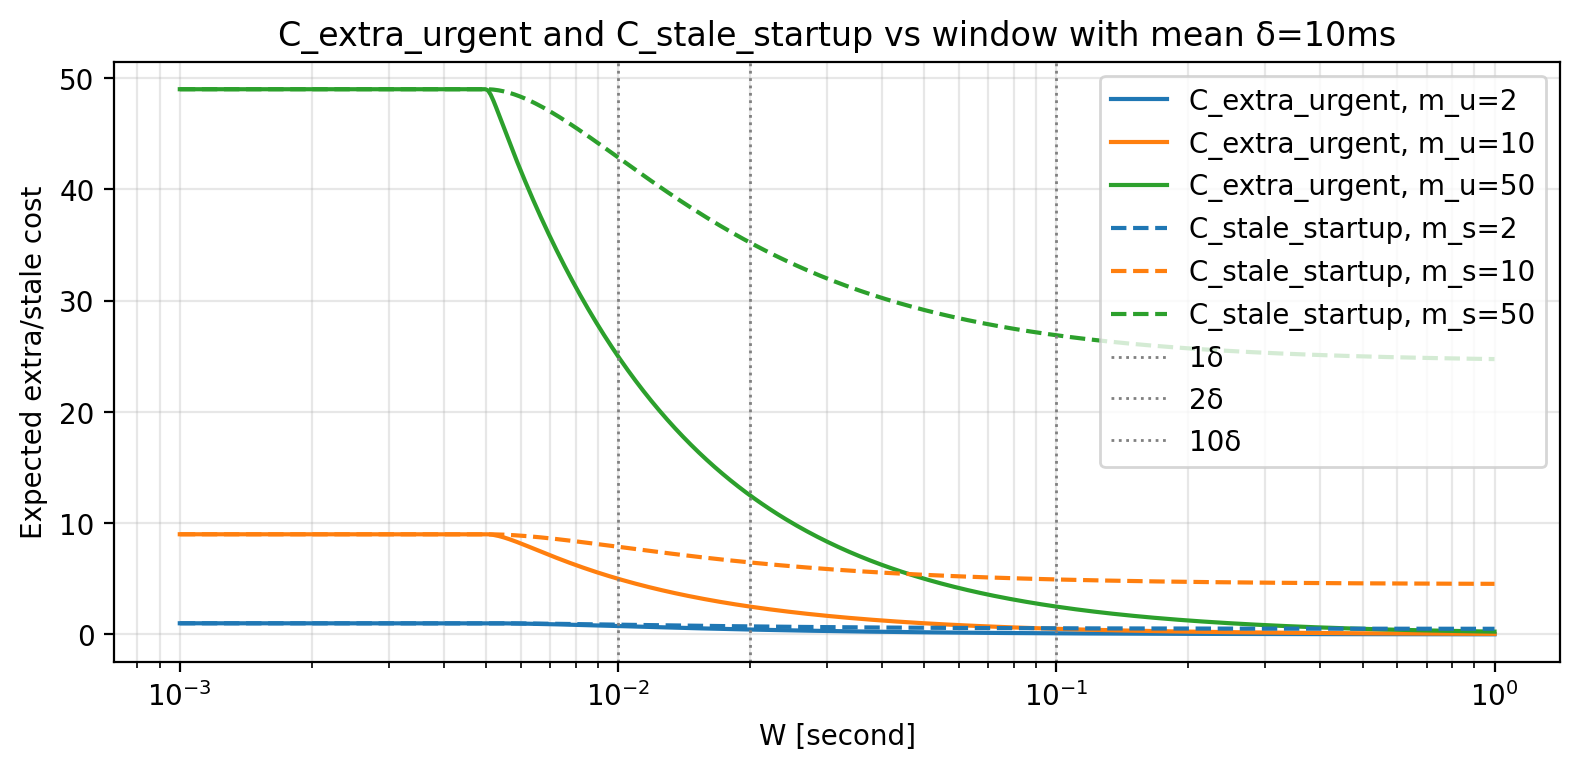
\includegraphics[width=0.85\textwidth]{appendices/randomized_gossip_delays.png}
    \caption{Expected extra urgent and stale startup gossips versus window
        length for several contender counts $m$, at
        $\delta = 10$~ms}
    \label{fig:appendix_gossip_delays_plot}
\end{figure}

The model produces the following guidance, which motivates the recommended
values in section~\ref{sec:session_parameters}:

\begin{itemize}
    \item $W_u$ should be on the order of $m_u \cdot \delta_{\max}$. Since
    $m_u$ is typically small, choosing
    $W_u \approx \delta_{\max}$ is usually sufficient.
    \item The benefit of increasing $W_s$ saturates quickly because the
    first term of $\mathbb{E}[C_{\text{stale,startup}}]$ is independent of
    $W_s$. Sensible values fall in the range
    $\delta_{\max} \lesssim W_s \lesssim 10\,\delta_{\max}$.
\end{itemize}

\begin{remark}
    An interesting direction for future refinement would be to downscale
    $W_u$ and $W_s$ with the number of local collisions observed, so that
    nodes with more extensive local allocation tables (oracle nodes) are
    more likely to gossip first. This is out of scope for the present
    specification.
\end{remark}
